\documentclass[12pt]{article}

% The preceding line is only needed to identify funding in the first footnote. If that is unneeded, please comment it out.
\usepackage{cite}
\usepackage{amsmath,amssymb,amsfonts}
\usepackage{algorithm}
\usepackage{algorithmic}
\usepackage{graphicx}
\usepackage{textcomp}
\usepackage{xcolor}
\usepackage{colortbl}
\usepackage{float}
\usepackage{subcaption}
\usepackage{multirow}

\def\BibTeX{{\rm B\kern-.05em{\sc i\kern-.025em b}\kern-.08em
    T\kern-.1667em\lower.7ex\hbox{E}\kern-.125emX}}
\begin{document}

\title{Coursework of Image Processing and computer vision}



\author{Chen Ting Hung}
	
\maketitle

\begin{abstract}
This report is trying to explain how the couseworkd implement some knowledge in digital image processing to detect edge, object throught the viola jones, sobel.
\end{abstract}

\section{Subtask 1}

%Annotate the test images to generate ground truth, then test the face detector’s performance (with the given parameters as provided by face.cpp) on five given example images: dart4.jpg, dart5.jpg, dart13.jpg, dart14.jpg and dart15.jpg. Produce the five result images with bounding boxes drawn around detected face candidates and include them in your report.

The results of task1 show in below Figure1. Red rectangel is drawn by myself and Green box is detected by computer via given frontalface.xml.\\

\begin{figure}[htb]
\centering
\begin{subfigure}[b]{.48\linewidth}
  \centering
  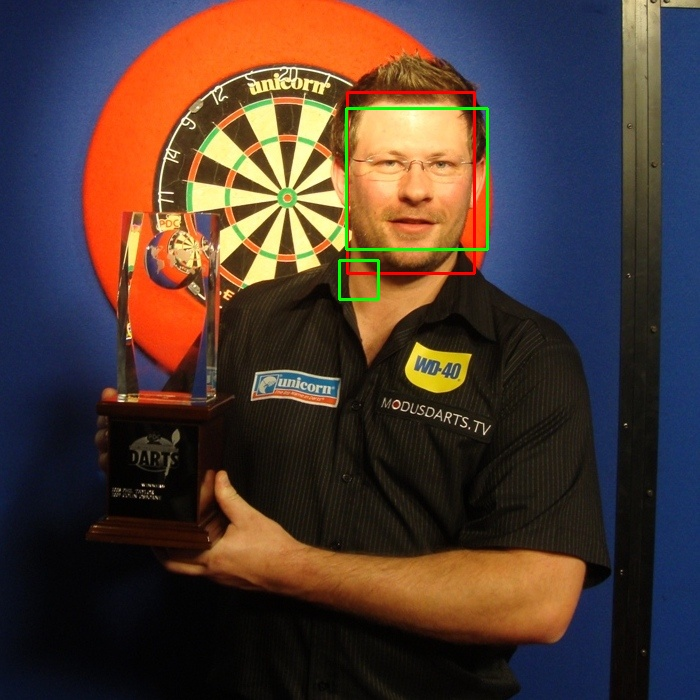
\includegraphics[width=\linewidth]{task1/result/dart4_detected.jpg}
  \caption{\textbf{\texttt{dart4.jpg}}}
\end{subfigure}
\begin{subfigure}[b]{.48\linewidth}
  \centering
  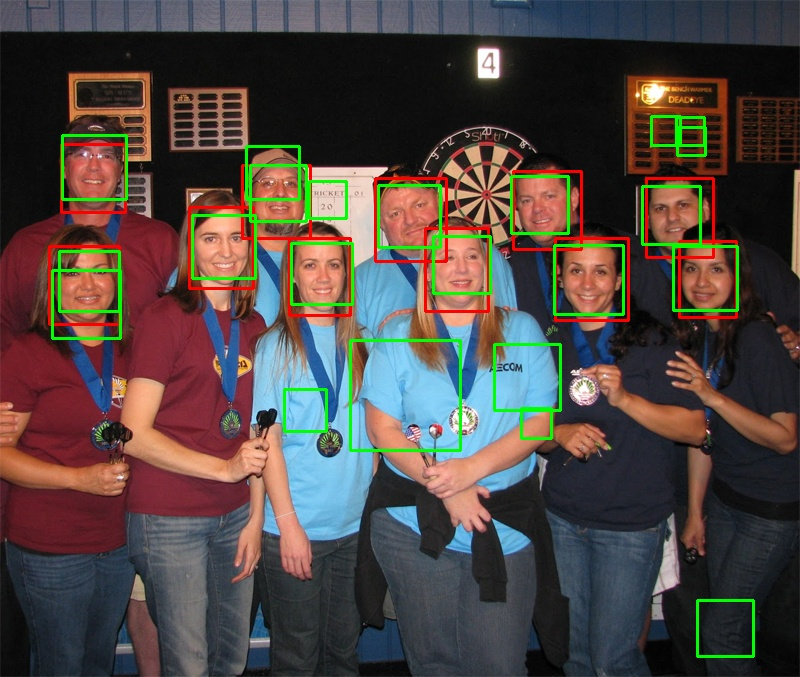
\includegraphics[width=\linewidth]{task1/result/dart5_detected.jpg}
  \caption{\textbf{\texttt{dart5.jpg}}}
\end{subfigure}
\begin{subfigure}[b]{.48\linewidth}
  \centering
  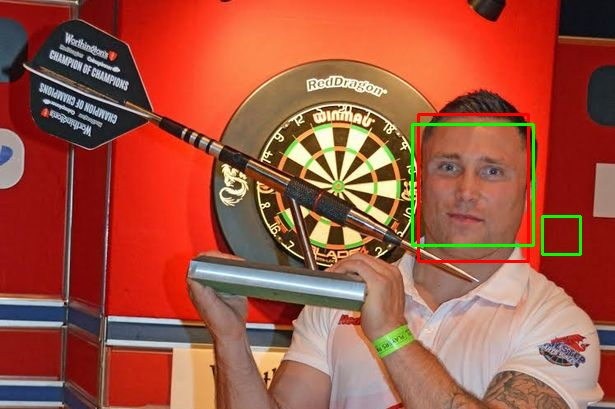
\includegraphics[width=\linewidth]{task1/result/dart13_detected.jpg}
  \caption{\textbf{\texttt{dart13.jpg}}}
\end{subfigure}
\begin{subfigure}[b]{.48\linewidth}
  \centering
  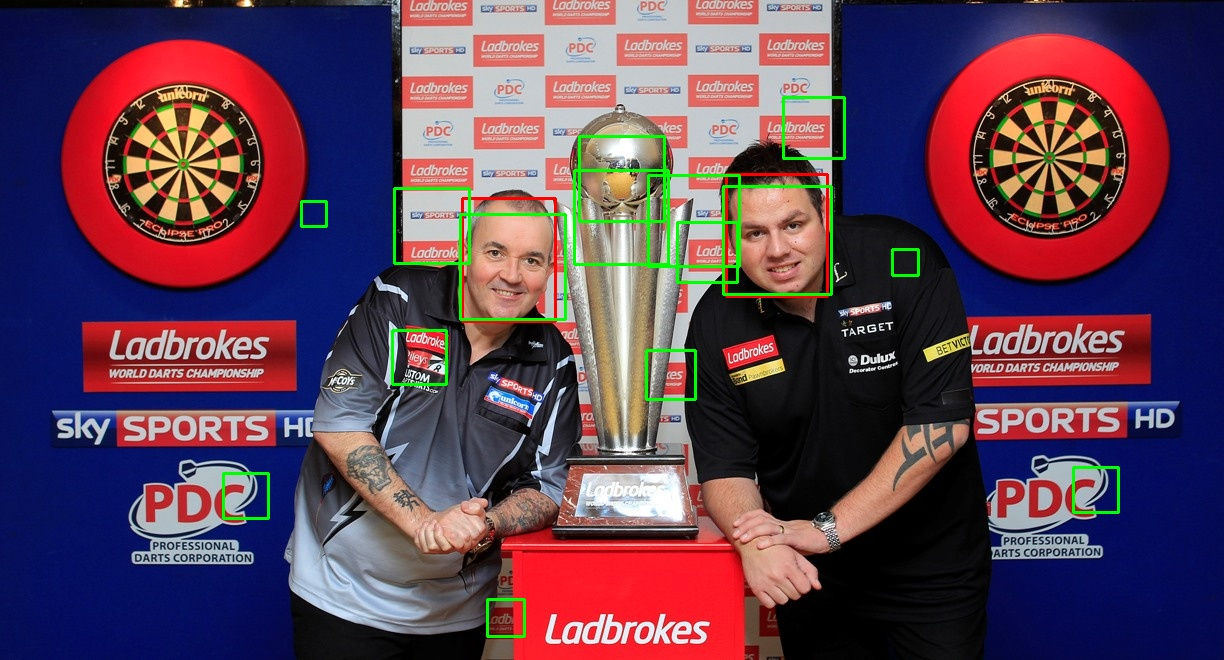
\includegraphics[width=\linewidth]{task1/result/dart14_detected.jpg}
  \caption{\textbf{\texttt{dart14.jpg}}}
\end{subfigure}
\begin{subfigure}[b]{.68\linewidth}
  \centering
  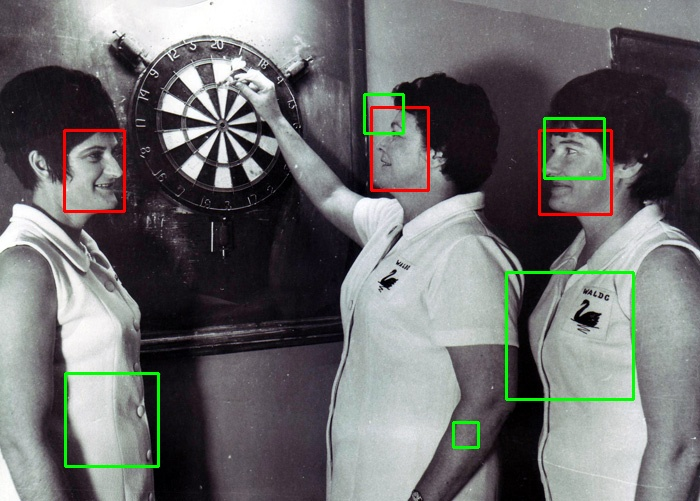
\includegraphics[width=\linewidth]{task1/result/dart15_detected.jpg}
  \caption{\textbf{\texttt{dart15.jpg}}}
\end{subfigure}
\label{fig:1}
\end{figure}

%b) Calculate and note in your report the TPR (true positive rate) for the images dart5.jpg and dart15.jpg, that is the fraction of successfully detected faces out of all valid faces in an image. Discuss in your team and briefly note in your report 1) some practical difficulties in assessing the TPR accurately, 2) why it is always possible to achieve a TPR of 100% on any detection task, and 3) implement a small piece of code to calculate the F1-score of your face detection system accurately and meaningfully from ground truth and a test run on any given test image set.

The true positive rate (TPR) for images dart5 is 11/16 and dart15 is 1/2.\\

The difficulty of assessing TPR accurately is that the truth image is drawn by manually and it is flexible not  absoulte so it is quiet difficult to assessing TPR.\\

F1 score is calculated by $(2*TP)/(2*TP+FN+FP)$  and f1 socre of dart5 and dart15 are 0.7058, 0.2352.\\

\clearpage

\section{Subtask 2}

%The training tool produces a strong classifier in stages. Per stage the tool adds further features to the classifier and prints the achieved TPR and FPR (false positive rate) for that point on the training data (see Figure). Collate this information into a scatter plot that plots TPR vs FPR on the training data for the three different stages. Produce this graph in your report and briefly interpret what it shows.

Figure2 \ref{fig:2} shows TPR and FPR. Three different stages of TPR are all 1.00 and 
FPR are 1, 0.0479088, 0.00437382 respectevely. The FPR become bigger when the stage increase.

\begin{figure}[htb]
	\centering
	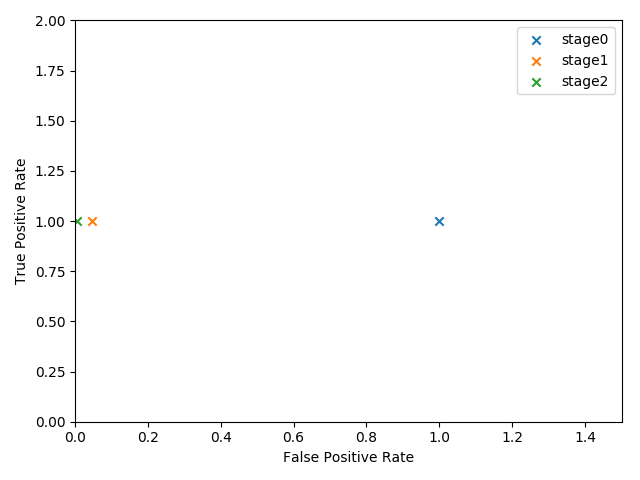
\includegraphics[width=\linewidth]{task2/result/plot.png}
	\caption{TPR and FPR.}
	\label{fig:2}
\end{figure}


Figure \ref{fig:3} shows four examples of test images using the 3-stage classifier. 

\begin{figure}[htb]
	\centering
	\begin{subfigure}[b]{.48\linewidth}
		\centering
		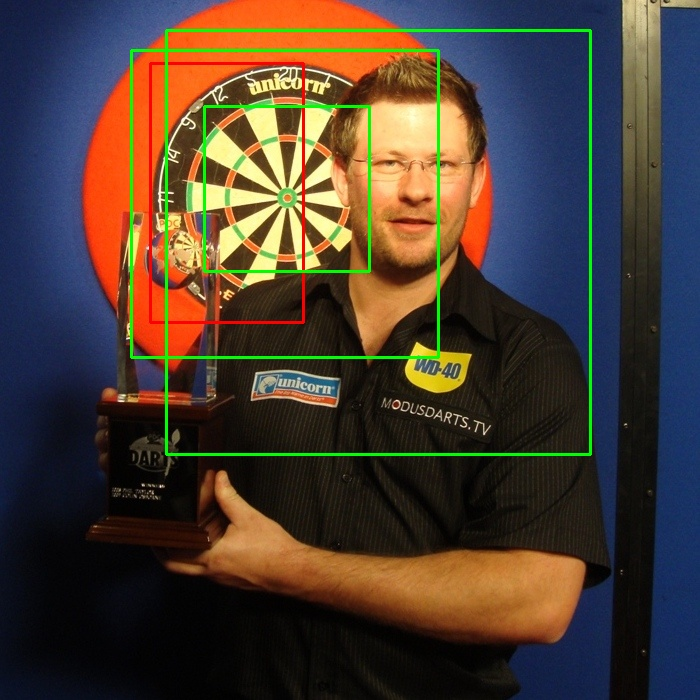
\includegraphics[width=\linewidth]{task2/result/dart4_detected.jpg}
		\caption{\textbf{\texttt{dart4.jpg}}}
	\end{subfigure}
	\begin{subfigure}[b]{.48\linewidth}
		\centering
		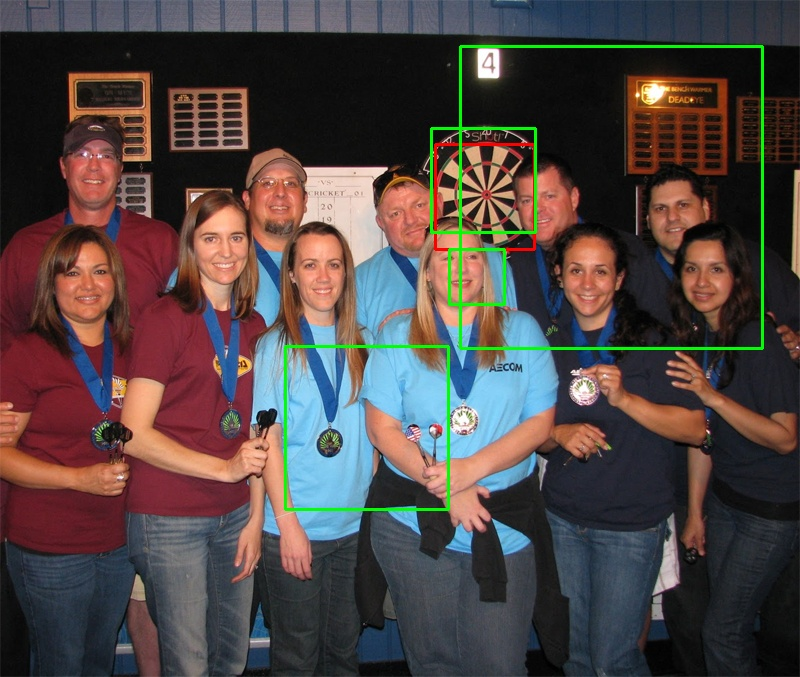
\includegraphics[width=\linewidth]{task2/result/dart5_detected.jpg}
		\caption{\textbf{\texttt{dart5.jpg}}}
	\end{subfigure}
	\begin{subfigure}[b]{.48\linewidth}
		\centering
		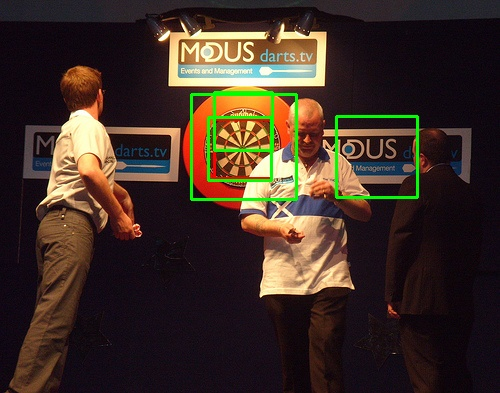
\includegraphics[width=\linewidth]{task2/result/dart6_detected.jpg}
		\caption{\textbf{\texttt{dart6.jpg}}}
	\end{subfigure}
	\begin{subfigure}[b]{.48\linewidth}
		\centering
		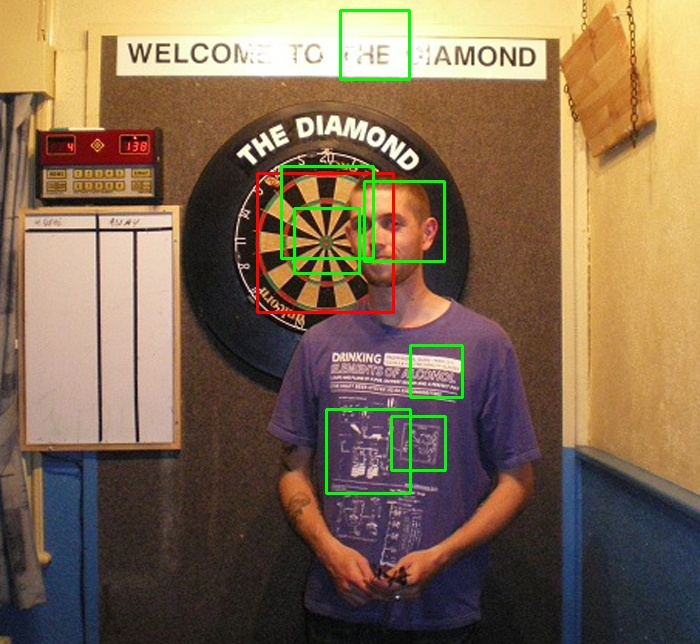
\includegraphics[width=\linewidth]{task2/result/dart7_detected.jpg}
		\caption{\textbf{\texttt{dart7.jpg}}}
	\end{subfigure}
	\caption{Detect dartboard }
	\label{fig:3}
\end{figure}


Table \ref{my-label} summarises the results of the classifier performance against all 16 test images for each of the training stages.

\begin{table}[htb]
	\centering
	\begin{tabular}{|l|llll|llll|}
		\hline
		\multirow{3}{*} & \multicolumn{1}{c|}{\textbf{F1 Score}} \\ \cline{2-9} 
		
		dart0.jpg & 0 \\
		dart1.jpg & 0   \\
		dart2.jpg & 0  \\
		dart3.jpg & 0  \\
		dart4.jpg & 0  \\
		dart5.jpg & 0.4 \\
		dart6.jpg & 0.4  \\
		dart7.jpg & 0.0  \\
		dart8.jpg & 0.5  \\
		dart9.jpg & 0.2857  \\
		dart10.jpg & 0  \\
		dart11.jpg & 0.4  \\
		dart12.jpg & 0  \\
		dart13.jpg & 0  \\
		dart14.jpg & 0   \\
		dart15.jpg & 0   \\ \hline
		\textbf{average} & \textbf{0.124}   \\ \hline
	\end{tabular}
	\caption{F1 scores.}
	\label{my-label}
\end{table}

\clearpage

\section{Subtask 3}

Figure \ref{fig:4} shows four best exhibit of test images 
\begin{figure}[htb]
	\centering
	\begin{subfigure}[b]{.48\linewidth}
		\centering
		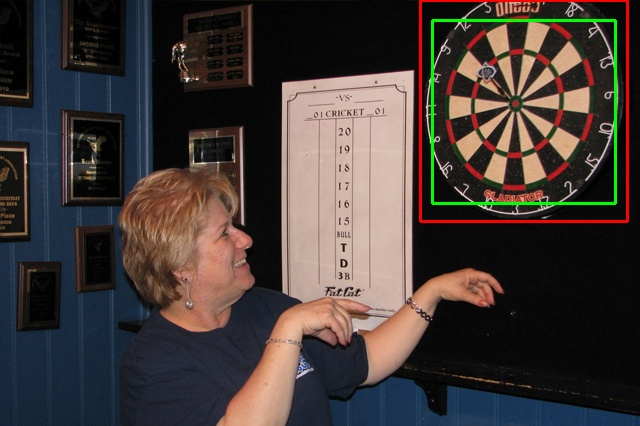
\includegraphics[width=\linewidth]{task3/result/dart0_detected.jpg}
		\caption{\textbf{\texttt{dart4.jpg}}}
	\end{subfigure}
	\begin{subfigure}[b]{.48\linewidth}
		\centering
		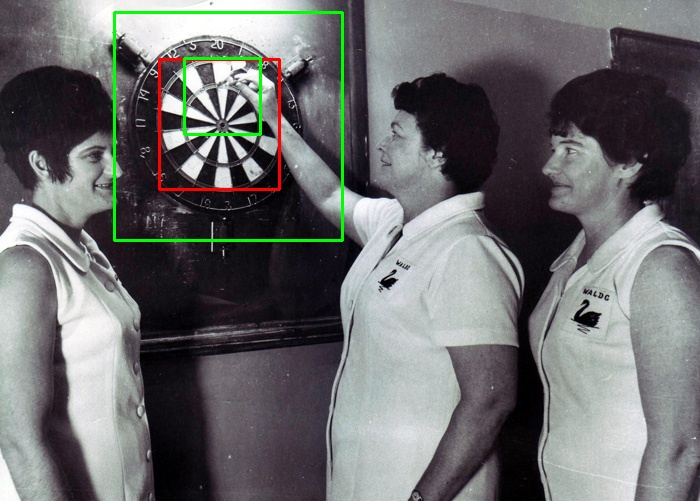
\includegraphics[width=\linewidth]{task3/result/dart15_detected.jpg}
		\caption{\textbf{\texttt{dart15.jpg}}}
	\end{subfigure}
	\caption{Detect dartboard with hough circle transform}
	\label{fig:4}
\end{figure}


c) In a flow diagram, depict how you have combined evidence from the Hough Transform and Viola-Jones detector. In bullet points, explain briefly your rationale behind the way you have combined evidence.\\

Answer: \\
1. I transform image to binary and use sobel to detect edges.\\
2. I used hough transform to detect the central point of circle.\\
3. I used central point and task2 result to check if central point is inside the result of task2\\


\section{Subtask 4}

a) In bullet points, explain briefly your rationale behind selecting the approach you have taken.\

Answer: \\
1. I adjust the kernal size of sobel from 5 to 3
1. I used binary image to detect the white space and draw a circle to magnify the feature\\
2. I transform image to binary and use sobel to detect edges.\\
3. I used hough transform to detect the central point of circle.\\
4. I used central point and task2 result to check if central point is inside the result of task2\\

b) Visualize important aspects of your technique in two of the given example dart images selected to best exhibit the merit of your approach.\\

Figure \ref{fig:5} shows four best exhibit of test images 
\begin{figure}[htb]
	\centering
	\begin{subfigure}[b]{.48\linewidth}
		\centering
		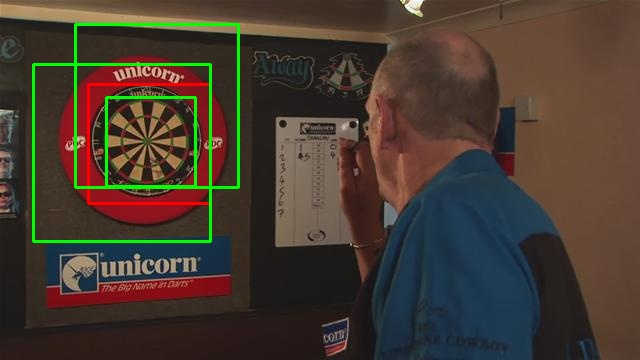
\includegraphics[width=\linewidth]{task4/result/dart2_detected.jpg}
		\caption{\textbf{\texttt{dart2.jpg}}}
	\end{subfigure}
	\begin{subfigure}[b]{.48\linewidth}
		\centering
		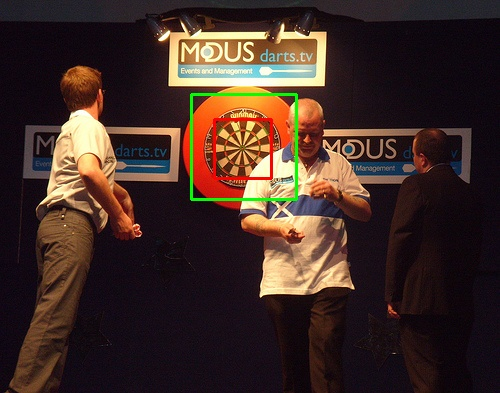
\includegraphics[width=\linewidth]{task4/result/dart6_detected.jpg}
		\caption{\textbf{\texttt{dart6.jpg}}}
	\end{subfigure}
	\caption{Detect dartboard with hough circle transform2}
	\label{fig:5}
\end{figure}

c) Evaluate your final detector on all of the example images, show the improvements in F1-score. Document your overall detection results and briefly note in bullet points the key merits and shortcomings of your final implementation.\\

Table \ref{my-label} summarises the results of the classifier performance against all 16 test images for each of the training stages.

\begin{table}[htb]
	\centering
	\begin{tabular}{|l|llll|llll|}
		\hline
		\multirow{3}{*} & \multicolumn{1}{c|}{\textbf{F1 Score}} \\ \cline{2-9} 
		
		dart0.jpg & 1 \\
		dart1.jpg & 0   \\
		dart2.jpg & 0.22  \\
		dart3.jpg & 0.4  \\
		dart4.jpg & 0  \\
		dart5.jpg & 0.4 \\
		dart6.jpg & 0.4  \\
		dart7.jpg & 0  \\
		dart8.jpg & 0.5  \\
		dart9.jpg & 0.28  \\
		dart10.jpg & 0.15  \\
		dart11.jpg & 0.4 \\
		dart12.jpg & 0.66  \\
		dart13.jpg & 0  \\
		dart14.jpg & 0   \\
		dart15.jpg & 0   \\ \hline
		\textbf{average} & \textbf{0.2767}   \\ \hline
	\end{tabular}
	\caption{F1 scores.}
	\label{my-label}
\end{table}

\end{document}
